\documentclass[a4paper]{article}

\usepackage{tecnico_relatorio}

\usepackage{textcomp}
\usepackage[hypcap]{caption} % makes \ref point to top of figures and tables
\usepackage{rotating}

\begin{document}
	\trSetImage{img/tecnico_logo}{6cm} % Logotipo do Técnico
	\trSetSubject{Arquitecturas Avançadas de Computadores}
	\trSetType{Laboratório II}
	\trSetTitle{Descrição do Processador \textmu RISC a Funcionar em Pipeline}
	
	\trSetBoxStyle{0.3}
	
	\trSetAuthorNr{3}
	
	\trSetAuthors
		{
		Gonçalo Ribeiro
		
		73294
		}{
		Miguel Costa
		
		73359
		}{
		Rafael Gonçalves
		
		73786
		}
		
	\trSetProfessor{Prof. Leonel Sousa}
	
	\trMakeCover
	
	\tableofcontents
	\pagebreak
	
	\section{Introdução}
	
	Nesta parte do trabalho pretende-se que o processador descrito na primeira parte passe a ter funcionamento em \textit{pipeline}. Como visto nas aulas teóricas isto permitirá aumentar o número de instruções que são executas por ciclo de relógio -- IPC.
	
	No entanto, introduzir \textit{pipelining} acarreta problemas que não existiam na versão anterior. É agora preciso ter em conta a existência de conflitos de dados e conflitos de controlo. Para mitigar o impacto destes problemas são implementados circuitos de detecção para conflitos, \textit{forwarding} e previsão dinâmica de saltos.
	
	
	\section{Introdução de Registos de \textit{Pipelining}}
	
	O primeiro passo para garantir o funcionamento em \textit{pipeline} é colocar registos entre os vários andares do processador, i.e.\ introduzir registos entre IF e ID/RF, ID/RF e EX/MEM e entre EX/MEM e WB.
	
	Estes registos já constavam da descrição do processador entregue na primeira parte deste trabalho. Deste modo, relativamente a estes registos bastou fazer com que os seus sinais de \textit{enable} sejam agora controlados pelo próprio processador e não por uma máquina de estados externa, como era feito na primeira parte do trabalho. Na \autoref{fig:circuit_pt1} recorda-se o circuito do processador descrito na primeira parte do projecto.
	
		\begin{figure}[h]
			\centering
			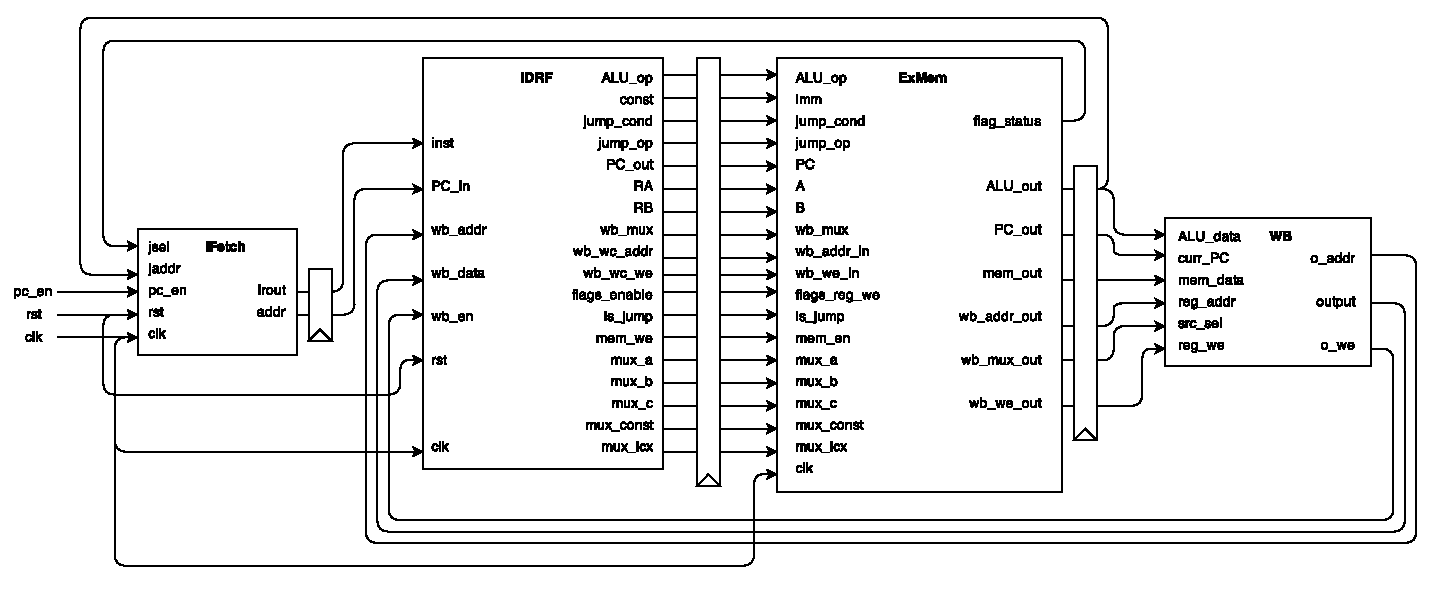
\includegraphics[width=1.\textwidth]{img/circuit_pt1}
			\caption{Circuito do \textmu RISC na primeira parte do trabalho. Podem ser vistos os registo entre andares}
			\label{fig:circuit_pt1}
		\end{figure}
	
	\section{Escrita Transparente do \textit{Register File}}
	
	Uma forma muito simples de começar a mitigar os conflitos de dados é alterar o flanco em que o \textit{Register Rile} é escrito.
	
	Na primeira parte do trabalho o RF era escrito sempre no flanco de relógio ascendente. Com a introdução do funcionamento em \textit{pipeline}, isto obriga a fazer um \textit{stall} sempre que num mesmo ciclo o WB for escrever num registo R$x$ e em ID/RF estiver a ser feito \textit{fetch} do valor de R$x$.
	
	Para resolver este problema o RF passa a ser escrito no flanco de relógio descendente. Assim, quando R$x$ é lido (no flanco ascendente) o valor de R$x$ já foi actualizado no flanco descendente, pelo que não é necessário atrasar a execução da instrução que está a ler o operando R$x$.
	
	\section{Detecção de Conflitos de Dados}
	
	\section{\textit{Forwarding}}
	
	\section{Testes e Simulações}
		
	\section{Conclusão}

\end{document}








